\section{The Approach}

\subsection{The Basic Idea: Combine GAS with Node Partitioning}

\begin{frame}
  \frametitle{The GAS Decomposition}
  The authors observed this pattern across many vertex programs.
  \begin{itemize}
    \item \textbf{Gather} an accumulated results from neighborhood.
    \item \textbf{Apply} the gathered result on the center node.
    \item \textbf{Scatter} accumulated information across the neighborhood.
  \end{itemize}
\end{frame}

\begin{frame}
  \frametitle{Node Partitioning}
  \begin{figure}
    \centering
    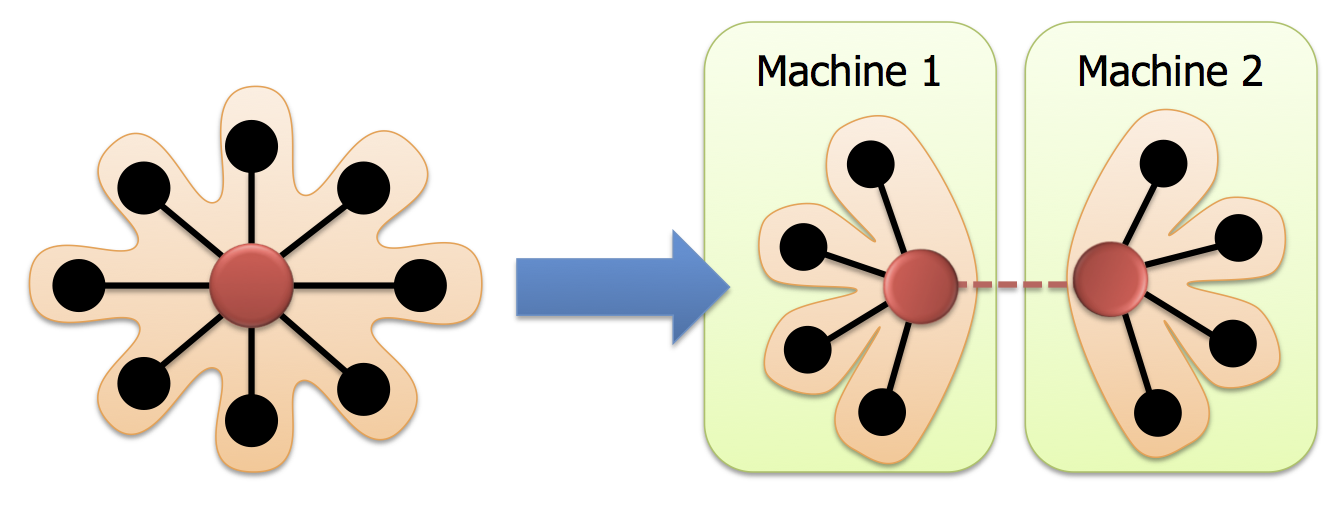
\includegraphics[scale=0.37]{gonzalez_osdi_2012_slide_13_simple}
    \caption{\cite[OSDI '12 Slides]{gonzalez2012powergraph-slides}}
  \end{figure}
\end{frame}

\begin{frame}
  \frametitle{The Key to Graph-Parallel Optimizations}
  \centering
  Parallelize vertex programs but also be able to parallelize their
  sub-operations: scatter and gather.
  \begin{figure}
    \centering
    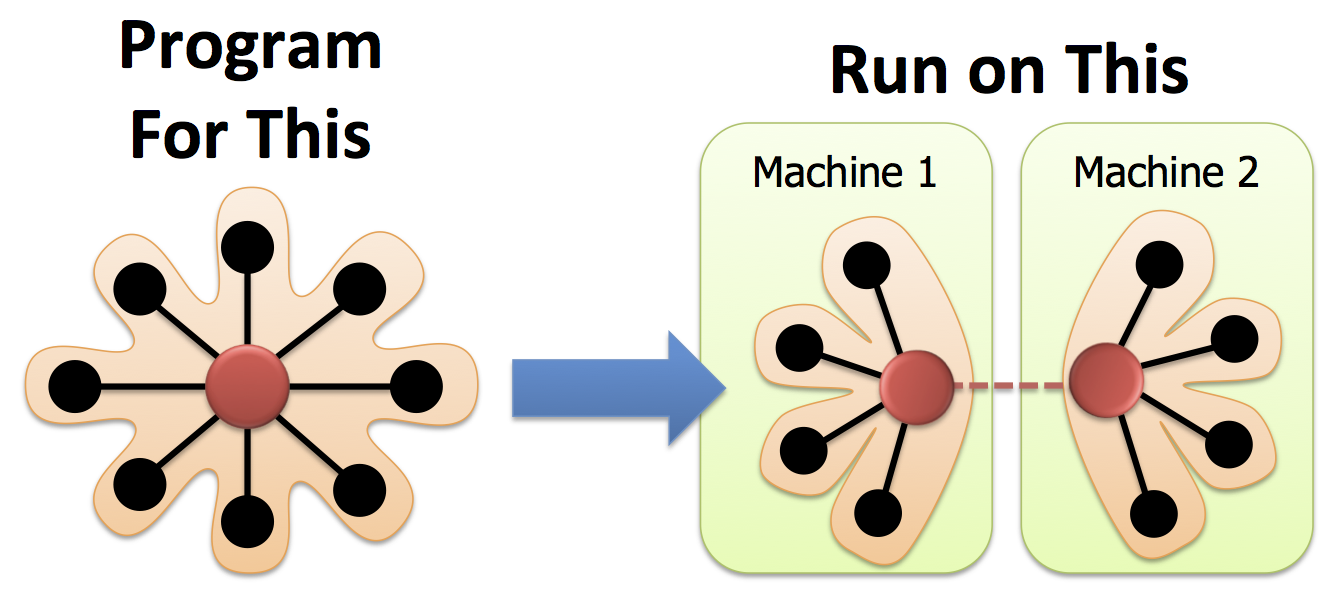
\includegraphics[scale=0.37]{gonzalez_osdi_2012_slide_13}
    \caption{\cite[OSDI '12 Slides]{gonzalez2012powergraph-slides}}
  \end{figure}
\end{frame}

\begin{frame}
  \frametitle{A Taste of the Results}
  \begin{figure}
    \centering
    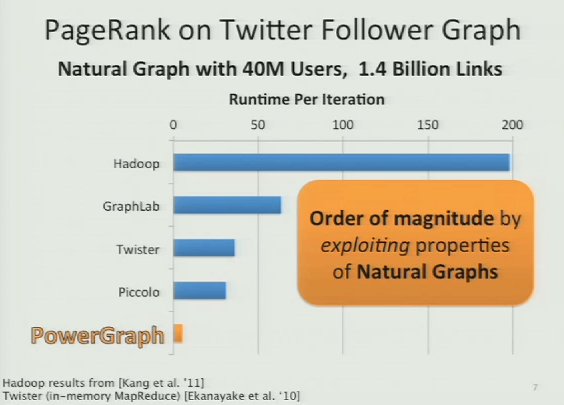
\includegraphics[scale=0.40]{gonzalez_osdi_2012_slide_7}
    \caption{\cite[OSDI '12 Slides]{gonzalez2012powergraph-slides}}
  \end{figure}
\end{frame}


\subsection{The PowerGraph Abstraction}

\begin{frame}
  \frametitle{The GAS Decomposition}
  \begin{figure}
    \centering
    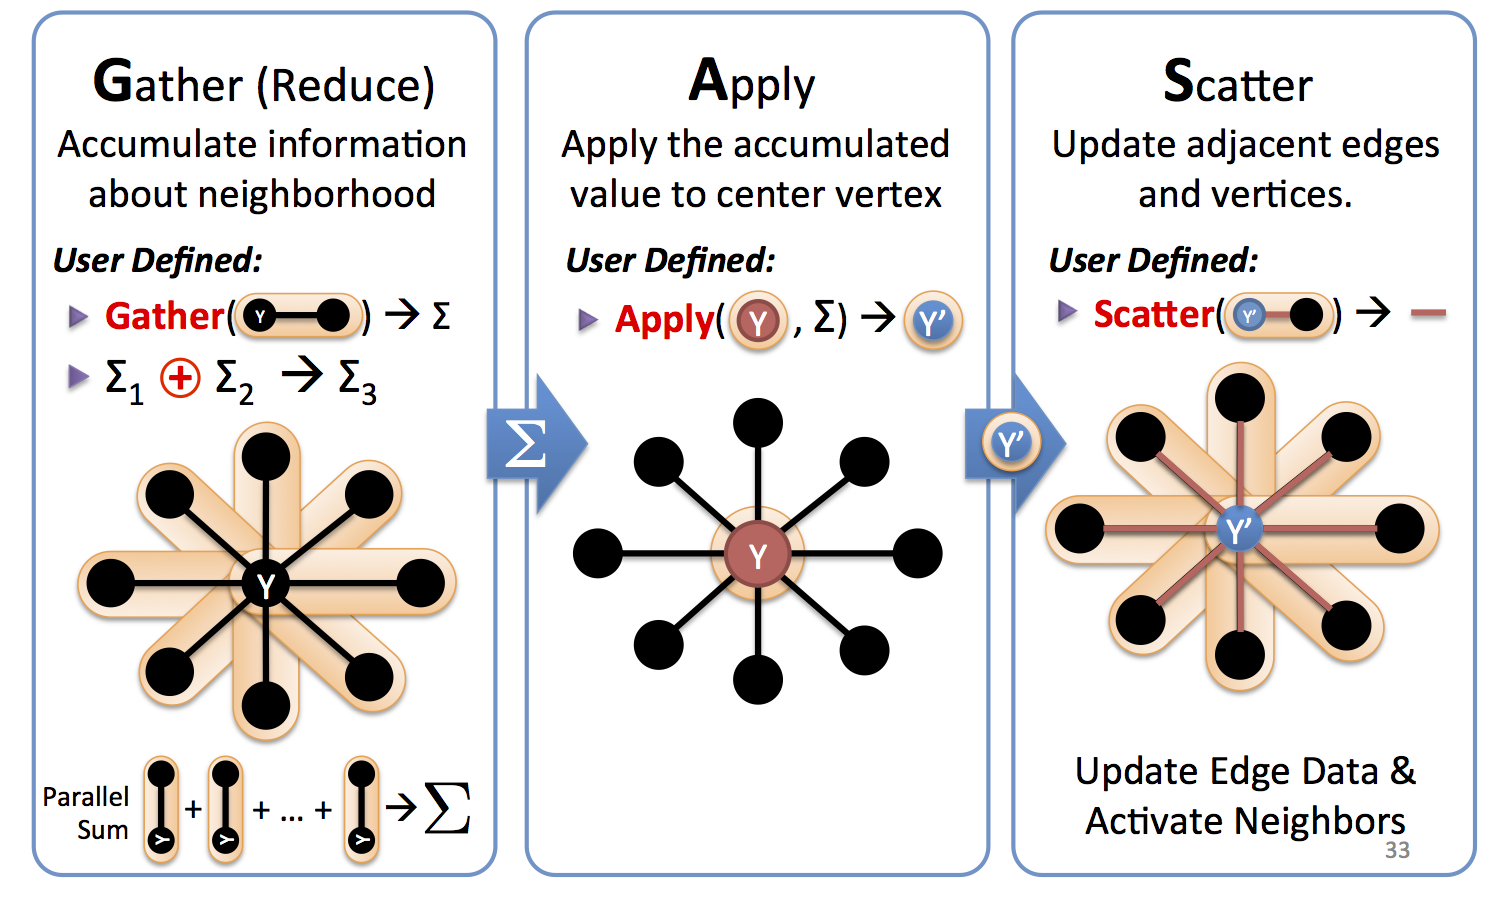
\includegraphics[scale=0.34]{gonzalez_osdi_2012_slide_33}
    \caption{\cite[OSDI '12 Slides]{gonzalez2012powergraph-slides}}
  \end{figure}
\end{frame}

\begin{frame}
  \frametitle{The PowerGraph Abstraction}
  PowerGraph lifts the GAS decomposition into the framework. The user implements
  each of these to make a vertex program.
  \begin{figure}
    \centering
    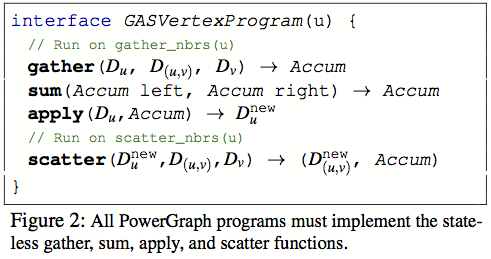
\includegraphics[scale=0.75]{gonzalez_osdi_2012_figure_2}
    \caption{\cite[OSDI '12]{gonzalez2012powergraph}}
  \end{figure}
\end{frame}

\begin{frame}
  \frametitle{Delta Caching}
  \textbf{TODO:} Everything!
\end{frame}

\begin{frame}
  \frametitle{Sequential Semantics}
  The meaning of a vertex program given the user-defined ops:
  \begin{figure}
    \centering
    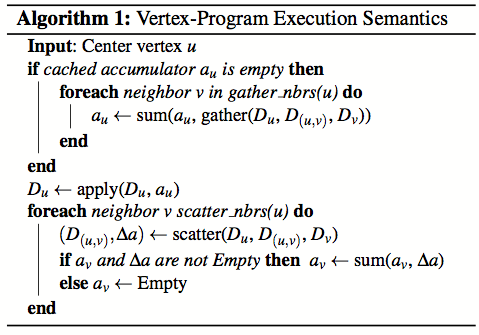
\includegraphics[scale=0.80]{gonzalez_osdi_2012_algorithm_1}
    \caption{\cite[OSDI '12]{gonzalez2012powergraph}}
  \end{figure}
\end{frame}



\subsection{Distributing the Graph and Computation}

\begin{frame}
  \frametitle{Edge-Cut vs Node-Cut Graph Partitioning}
  \begin{figure}
    \centering
    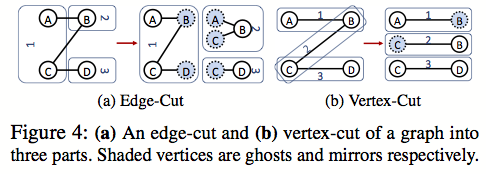
\includegraphics[scale=1.0]{gonzalez_osdi_2012_figure_4}
    \caption{\cite[OSDI '12]{gonzalez2012powergraph}}
  \end{figure}
\end{frame}

\begin{frame}
  \frametitle{A Vertex Program on a Cut Vertex}
  \begin{figure}
    \centering
    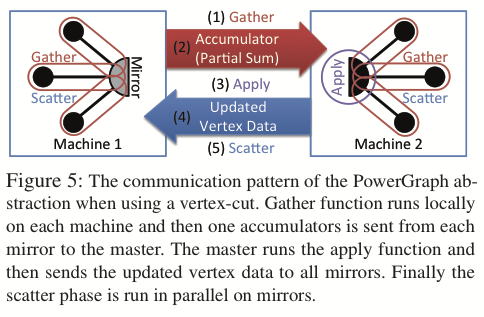
\includegraphics[scale=0.95]{gonzalez_osdi_2012_figure_5}
    \caption{\cite[OSDI '12]{gonzalez2012powergraph}}
  \end{figure}
\end{frame}


\subsection{An Example Vertex Program}

\begin{frame}
  \frametitle{\textit{Example:} Greedy Graph Coloring}
  \begin{figure}
    \centering
    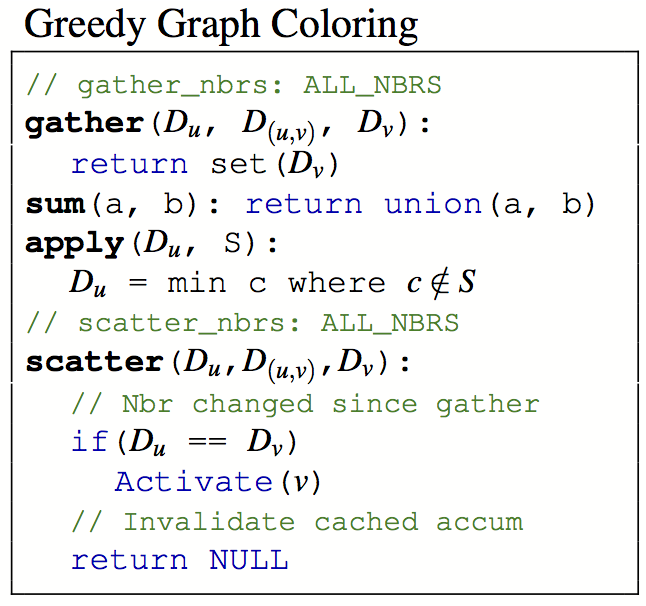
\includegraphics[scale=1.0]{gonzalez_osdi_2012_figure_3b}
    \caption{\cite[OSDI '12]{gonzalez2012powergraph}}
  \end{figure}
\end{frame}


\subsection{Limitations}

\begin{frame}
  \frametitle{Limitations of Approach}
  \begin{itemize}
    \item Static graph topology.
    \item TODO?
  \end{itemize}
\end{frame}

\begin{frame}
\begin{itemize}
  \item % TODO What was our solution
\end{itemize}
\end{frame}
